\begin{figure}[h!]
	\centering
	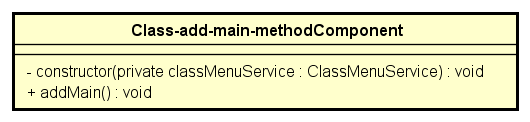
\includegraphics[scale=0.8]{res/sections/SpecificaFrontEnd/Components/Disegnetti/class-add-main-method.png}
	\caption{Diagramma della classe Class-add-main-method}
\end{figure}

\begin{itemize}
	\item \textbf{Descrizione:}\\
	Gestisce l'aggiunta di un metodo main alla classe.
	\item \textbf{Utilizzo:}\\
	Viene utilizzata dal EditClassMenuComponent per la gestione dell'aggiunta del main a una classe.
	\item \textbf{Metodi:}
		\begin{itemize}
			\item \emph{-constructor(private classMenuService: ClassMenuService)}\\
    		Costruttore della classe\\
    		\textbf{Parametri:}
    		\begin{itemize}
    			\item \emph{classMenuService: ClassMenuService}\\
    			Crea un istanziazione di ClassMenuService
    		\end{itemize}
    		\item \emph{addMain()}\\
    		Aggiunge il metodo main alla classe selezionata
		\end{itemize}
\end{itemize}